\chapter{Implementasi, Pengujian dan Eksperimen}
\section{Deskripsi Perangkat Keras dan Lunak yang Digunakan}
\label{sec:deskripsi_perangkat_keras}
Pada penelitian ini terdapat dua tahap implementasi. Implementasi pertama dilakukan di komputer peneliti untuk keperluan pengujian fungsional. Komputer tersebut memiliki spesifikasi sebagai berikut:

\begin{enumerate}
	\item Processor: 2.5 GHz Intel Core i5
	\item RAM: 10 GB DDR3
	\item Sistem Operasi: OS X El Capitan (v10.11.3)
	\item Versi Java: 1.8.0\_45
	\item Apache Hadoop: 2.7.1
	\item Apache Hive: 1.2.1
	\item Apache Sqoop: 1.4.6
	\item MySQL: 5.5.40
	\item Pentaho Data Integration (PDI): Community Edition 6.0.1.0
\end{enumerate}

Implementasi kedua dilakukan pada komputer laboratorium untuk pengujian eksperimental. Jumlah total komputer yang digunakan untuk eksperimen adalah 1 buah komputer \textit{master} dan 25 komputer \textit{slave}. Komputer-komputer tersebut memiliki spesifikasi sebagai berikut:
\begin{enumerate}
	\item Processor: 3.3 GHz Intel Core i3
	\item RAM: 4 GB DDR3
	\item Sistem Operasi: Ubuntu 14.04 LTS
	\item Versi Java: 1.8.0\_45
	\item Apache Hadoop: 2.7.1
	\item Apache Hive: 1.2.1
	\item Apache Sqoop: 1.4.6
	\item MySQL: 5.5.40
	\item Pentaho Data Integration (PDI): Community Edition 6.0.1.0
\end{enumerate}

\section{Implementasi Modul Program}
\subsection{Implementasi Modul Program \textit{Streaming} Twitter}
Implementasi modul program \textit{streaming} Twitter akan terbagi menjadi dua buah bagian yaitu implementasi antarmuka program dan implementasi kode di dalamnya. 

\subsubsection{Implementasi Antar Muka \textit{Streaming} Twitter}
Gambar \ref{fig:ui_implementasi_streaming_twitter} merupakan hasil implementasi dari modul program ini. Implementasi antarmuka modul program ini dibuat menggunakan Java Swing. 

Pengguna dapat memasukan data-data seperti consumer key, consumer secret, access token dan access token secret sesuai dengan data yang didapatkan dari Twitter Streaming API. Selain itu pengguna juga dapat memasukan kata kunci untuk mendapatkan \textit{tweet} yang relevan dengan kebutuhan organisasi. Untuk pilihan lokasi penyimpanan, pengguna dapat menggunakan \textit{radio button} dan mengisi lokasi \textit{path}.
 
\begin{figure}[H]
	\centering
	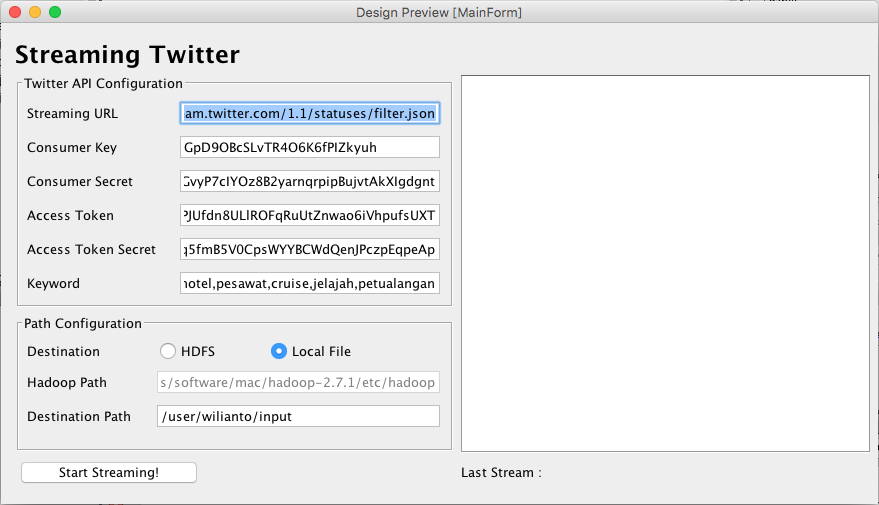
\includegraphics[scale=0.5]{Gambar/ui-implementasi-streaming-twitter.png}
	\caption[Implementasi Antarmuka \textit{Streaming} Twitterr]{Implementasi Antarmuka \textit{Streaming} Twitter} 
	\label{fig:ui_implementasi_streaming_twitter}
\end{figure}


\subsubsection{Implementasi Kode Program \textit{Streaming} Twitter}
Kode program pada modul ini ditulis menggunakan program Java. Berikut adalah potongan-potongan kode hasil implementasi dari modul progam ini. 

\begin{lstlisting}[language=Java,basicstyle=\tiny,caption=Writer.java,label={lst:kode_writer}]
public interface Writer {
    public void write(String path, String content);
    public void close();
}
\end{lstlisting}

\begin{lstlisting}[language=Java,basicstyle=\tiny,caption=LocalOperation.java,label={lst:kode_local_operation}]
public class LocalOperation implements Writer{
    protected String fileName;
    protected FileWriter fw;

    @Override
    public void write(String path, String content) {
        try {
            if(this.fw == null){
                this.fw = new FileWriter(path);
            }
            
            fw.append(content);
        } catch (IOException ex) {
            System.out.println(ex.toString());
        }
    }
    
    ....
}
\end{lstlisting}

\begin{lstlisting}[language=Java,basicstyle=\tiny,caption=HDFSOperation.java,label={lst:kode_hdfs_operation}]
public class HDFSOperation implements Writer{
    protected String hadoopPath;
    protected Configuration conf;
    protected FileSystem fs;
    
    protected void init(){
        conf = new Configuration();
        conf.addResource(new Path(hadoopPath + "/core-site.xml"));
        conf.addResource(new Path(hadoopPath + "/hdfs-site.xml"));
        conf.set("fs.hdfs.impl", org.apache.hadoop.hdfs.DistributedFileSystem.class.getName());
        conf.set("fs.file.impl", org.apache.hadoop.fs.LocalFileSystem.class.getName());
        try {
            fs = FileSystem.get(conf);
        } catch (IOException ex) {
            System.out.println(ex.getMessage());
        }
    }
    
    public void write(String hdfsPath, String content) {
        Path path = new Path(hdfsPath);
        try{
            FSDataOutputStream fos;
            //delete file if exist
            if(fs.exists(path)){
                fos = fs.append(path);
            }else{
                fos = fs.create(path);
            }
            
            //create file and write content to file
            fos.writeUTF(content);
            fos.close();
        }catch(IOException ex){
            System.out.println(ex.getMessage());
        }
    }
    
    public String read(String hdfsPath) {
        String content = null;
        Path path = new Path(hdfsPath);
        try{
            //create file and write content to file
            FSDataInputStream fis = fs.open(path);
            BufferedReader reader = new BufferedReader(new InputStreamReader(fis.getWrappedStream()));
            String s;
            while((s = reader.readLine()) != null){
                content += s;
            }
            reader.close();
            fis.close();
        }catch(IOException ex){
            System.out.println(ex.getMessage());
        }
        return content;
    }
    
    public void copyFromLocal(String localPath, String hdfsPath){
        Path srcPath = new Path(localPath);
        Path destPath = new Path(hdfsPath);
        
        try{
            //check is path exist
            if(fs.exists(destPath)){
                System.out.println("No such destination " + destPath);
                return;
            }
            
            fs.copyFromLocalFile(srcPath, destPath);
        }catch(IOException ex){
            System.out.println(ex.getMessage());
        }
    }
    
    public void delete(String hdfsPath) {
        Path path = new Path(hdfsPath);
        try{
            fs.delete(path, true);
        }catch(IOException ex){
            System.out.println(ex.getMessage());
        }
    }
    
    ....
}
\end{lstlisting}

\begin{lstlisting}[language=Java,basicstyle=\tiny,caption=TwitterStreamer.java,label={lst:kode_twitter_streamer}]

public class TwitterStreamer extends Thread {

    ....
    
    public TwitterStreamer(String streamUrl, String consumerKey, String consumerSecret, String accessToken, String accessTokenSecret, String keyword, String hadoopPath, String filePath, JTextArea textArea, JLabel lastStreamLabel) {
        
        ....
        
        if(this.hadoopPath != ""){
            this.writer = new HDFSOperation(hadoopPath);
        }else{
            this.writer = new LocalOperation();
        }
    }

    public void run() {
        try {
            OAuthService service = new ServiceBuilder()
                    .provider(TwitterApi.class)
                    .apiKey(consumerKey)
                    .apiSecret(consumerSecret)
                    .build();

            //set access token
            textArea.setText("Started...\n");
            Token accessTokenGenerated = new Token(accessToken, accessTokenSecret);

            //generate the request
            OAuthRequest request = new OAuthRequest(Verb.POST, streamUrl);
            request.addHeader("version", "HTTP/1.1");
            request.addHeader("host", "stream.twitter.com");
            request.setConnectionKeepAlive(true);
            request.addHeader("user-agent", "Twitter Stream Reader");
            request.addBodyParameter("track", keyword); 
            request.addBodyParameter("language", "in");
            service.signRequest(accessTokenGenerated, request);
            Response response = request.send();
            
            BufferedReader reader = new BufferedReader(new InputStreamReader(response.getStream()));
            
            String line;
            JSONObject jsonObj;
            String sourceId, text, geo, place, timestampMs, appendLine;
            SimpleDateFormat sdf = new SimpleDateFormat("MMM dd,yyyy HH:mm:ss");    
            Date date;
            while ((line = reader.readLine()) != null && start) {
                try{
                    jsonObj = new JSONObject(line);
                    if(jsonObj.has("text") && jsonObj.get("text") != null){
                        sourceId = jsonObj.has("id_str") ? jsonObj.getString("id_str") : null;
                        text = jsonObj.has("text") ? jsonObj.getString("text") : null;
                        geo = jsonObj.has("geo") ? jsonObj.get("geo").toString() : null;
                        place = jsonObj.has("place") ? jsonObj.get("place").toString() : null;
                        timestampMs = jsonObj.has("timestamp_ms") ? jsonObj.getString("timestamp_ms") : null;
                        appendLine = sourceId + "\t" + text.replaceAll("\\n", " ") + "\t" + geo + "\t" + place + "\t" + timestampMs + "\t";
                        textArea.setText(counter + " data.");
                        writer.write(filePath, appendLine + "\n");
                        date = new Date(System.currentTimeMillis());
                        lastStreamLabel.setText(sdf.format(date));
                        counter++;
                    }
                }catch(Exception e){
                }
            }
            writer.close();
            textArea.setText(textArea.getText() + "Stopped...\n");
        } catch (IOException ex) {
            ex.printStackTrace();
        }
    }
    
    ....
}
\end{lstlisting}

\subsection{Implementasi Modul Program \textit{Crawling} Instagram}
Implementasi modul program \textit{crawling} Instagram akan terbagi menjadi dua buah bagian yaitu implementasi antarmuka program dan implementasi kode di dalamnya. 

\subsubsection{Implementasi Antar Muka \textit{Crawling} Instagram}
Gambar \ref{fig:ui_implementasi_streaming_instagram} merupakan hasil implementasi dari modul program ini. Implementasi antarmuka modul program ini dibuat menggunakan Java Swing. 

Pengguna dapat memasukan data-data seperti \textit{client ID, client secret} dan \textit{redirect URL} sesuai dengan data yang didapatkan dari Instagram API. Selain itu pengguna juga dapat memasukan tag untuk mendapatkan media dengan caption yang relevan dengan kebutuhan organisasi. Untuk pilihan lokasi penyimpanan, pengguna dapat menggunakan \textit{radio button} dan mengisi lokasi \textit{path}. Namun sebelum memulai pengguna harus mendapatkan \textit{code} terlebih dahulu dengan cara mengklik tombol "Get Code", lalu login dengan akun Instagramnya di browser. Setelah berhasil pengguna akan diarahkan ke sebuah halaman yang berisi \textit{code}.

\begin{figure}[H]
	\centering
	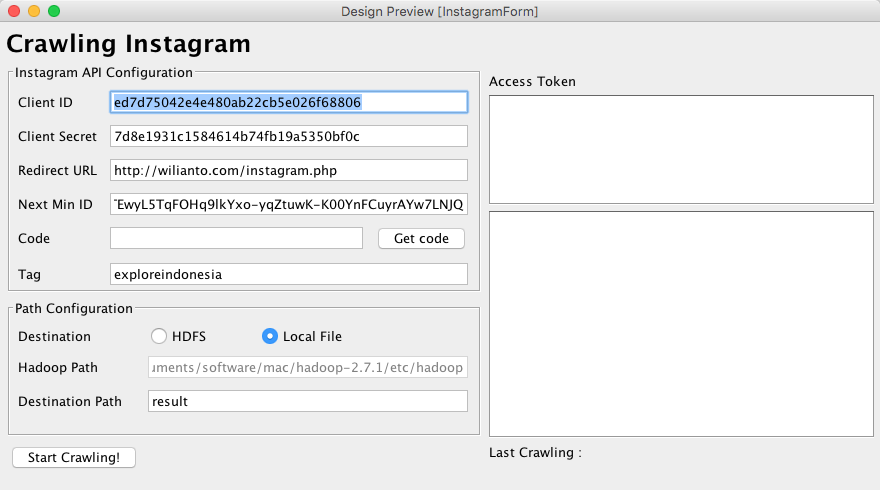
\includegraphics[scale=0.5]{Gambar/ui-implementasi-crawling-instagram.png}
	\caption[Implementasi Antarmuka \textit{Crawling} Instagram]{Implementasi Antarmuka \textit{Crawling} Instagram} 
	\label{fig:ui_implementasi_streaming_instagram}
\end{figure}

\subsubsection{Implementasi Kode Program \textit{Crawling} Instagram}
Kode program pada modul ini ditulis menggunakan program Java. Untuk kode Writer.java, HDFSOperation.java dan LocalOperation.java dapat dilihat pada Listing \ref{lst:kode_writer}, \ref{lst:kode_hdfs_operation} dan \ref{lst:kode_local_operation}. Berikut adalah kode-kode hasil implementasi dari modul progam ini. 

\begin{lstlisting}[language=Java,basicstyle=\tiny,caption=TwitterStreamer.java,label={lst:kode_instagram_crawler}]
public class InstagramCrawler extends Thread{
    ....
    
    public InstagramCrawler(String clientId, String clientSecret, String redirectUrl, String code, String nextMinId, String tag, String hadoopPath, String filePath, JTextArea textArea, JLabel lastStreamLabel, JTextField minTagIdTextField, JTextArea jsonTextArea, JButton triggerBtn, InstagramForm form) {
        ....
        
        if(this.hadoopPath != ""){
            this.writer = new HDFSOperation(hadoopPath);
        }else{
            this.writer = new LocalOperation();
        }
    }
    
    @Override
    public void run() {
        try {
            this.getAccessToken();
            writer.close();
            logWriter.close();
        } catch (IOException ex) {
            Logger.getLogger(InstagramCrawler.class.getName()).log(Level.SEVERE, null, ex);
        }
    }
    
    protected String generateUrl(){
        String url = "https://api.instagram.com/v1/tags/" + tag + "/media/recent"
                + "?count=100"
                + "&min_tag_id=" + nextMinId
                + "&access_token=" + accessToken;
        return url;
    }
    
    public void getAccessToken() throws MalformedURLException, IOException{
        this.start = true;
        triggerBtn.setText("Stop Crawling!");
        textArea.setText("Started...\n");
        
        if(this.accessToken == null || this.accessToken.isEmpty()){
            textArea.setText("Requesting access token...\n");

            //set URL
            url = new URL("https://api.instagram.com/oauth/access_token");

            //create connection with GET method
            conn = (HttpURLConnection) url.openConnection();
            conn.setRequestMethod("POST");
            //create data in URL format
            String data = "client_id=" + clientId
                    + "&client_secret=" + clientSecret
                    + "&grant_type=authorization_code"
                    + "&redirect_uri=" + redirectUrl
                    + "&code=" + code;

            //get output stream from connection to send the data
            conn.setDoOutput(true);
            OutputStream os = new BufferedOutputStream(conn.getOutputStream());
            os.write(data.getBytes());
            os.flush();
            os.close();

            //read the returned data
            br = new BufferedReader(new InputStreamReader(conn.getInputStream()));

            result = "";
            while((line = br.readLine()) != null){
                result += line;
            }
            json = new JSONObject(result);
            if(json.has("access_token")){
                this.accessToken = json.getString("access_token");
                jsonTextArea.setText(this.accessToken); 
                
                textArea.setText("Access token created...\n");
                this.getTagMediaRecent(this.generateUrl());
            }else{
                this.start = false;
                triggerBtn.setText("Start Crawling!");
                return;
            }
        }else{
            textArea.setText("Access token created...\n");
            this.getTagMediaRecent(this.generateUrl());
        }
    }
    
    public void getTagMediaRecent(String urlTagMediaRecent) 
            throws MalformedURLException, IOException {
        //set URL
        url = new URL(urlTagMediaRecent);

        //create connection with GET method
        conn = (HttpURLConnection) url.openConnection();
        conn.setRequestMethod("GET");

        //read the returned data
        br = new BufferedReader(new InputStreamReader(conn.getInputStream()));

        result = "";
        while((line = br.readLine()) != null){
            result += line;
        }

        //parse json object
        json = new JSONObject(result);
        datas = json.getJSONArray("data");

        for(int i = 0; i < datas.length(); i++){
            data = datas.getJSONObject(i);

            try{
                caption = (data.get("caption") != null) ? data.getJSONObject("caption") : null;
                location = (data.get("location") != null) ? data.get("location").toString() : null;
                locationName = (location != null) ? data.getJSONObject("location").getString("name") : "";
                text = caption != null ? caption.getString("text") : " ";
                text = text.replaceAll("\\n", " ");
                text = text + " " + locationName;
                //standard format with twitter streamer
                appendLine = "instagram-" + data.getString("id") + "\t" + text + "\t instagram \t" + location + "\t" + data.getString("created_time") + "000\t";
                textArea.setText(counter + " data.");
                writer.write(filePath, appendLine + "\n");
                date = new Date(System.currentTimeMillis());
                lastStreamLabel.setText(sdf.format(date));
                counter++;
            }catch(Exception ex){
            }
        }
        br.close();

        //do recursively
        pagination = json.getJSONObject("pagination");
        nextMinId = pagination.getString("next_min_id");
        nextUrl = pagination.has("next_url") ? pagination.getString("next_url") : null;
        logWriter.write("log.txt", sdf.format(date) + "\t" + tag + "\t" + nextMinId + "\n");

        if(nextUrl != null && start && counter < 15000){ 
            depth++;
            minTagIdTextField.setText(nextMinId);
            getTagMediaRecent(nextUrl);
        }else{
            minTagIdTextField.setText(nextMinId);
            textArea.setText(textArea.getText() + "\nStopped...");
            this.stopCrawling();
            //if not terminated by user, run new thread again
            if(!this.terminatedByUser){
                this.form.run();
            }
        }
    }
    
    ....
}
\end{lstlisting}

\subsection{Implementasi Modul Program Pembersihan Data dan Penghitungan Frekuensi Lokasi Wisata}
Implementasi pada modul ini dibuat menjadi dua buah program. Program utama menggunakan MapReduce sedangkan program kedua tanpa MapReduce. Tujuannya untuk mendapatkan hasil pengujian kedua buah program dari sisi waktu eksekusi. 

Potongan kode program pada Listing \ref{lst:kode_trie_node}, \ref{lst:kode_trie} dan \ref{lst:kode_cleaner} digunakan oleh kedua buah program. Listing \ref{lst:kode_trie_node} dan \ref{lst:kode_trie} merupakan kelas-kelas yang mengimplementasikan struktur data Trie yang sederhana untuk keperluan penyimpanan (\textit{dictionary}) kata lokasi wisata. Listing \ref{lst:kode_cleaner} merupakan implementasi kelas yang digunakan untuk melakukan pembersihan pada data sebelum diproses lebih lanjut.

Listing \ref{lst:kode_mapreduce} adalah potongan kode program yang menggunakan MapReduce. Pada kelas Map, dilakukan pembersihan data kemudian pencarian lokasi wisata yang terkandung di dalam data. Sedangkan pada kelas Reduce, dilakukan pengumpulan kata-kata hasil pencarian di Map dan dilakukan penghitungan frekuensi kemunculan kata di dalam suatu waktu.

Listing \ref{lst:kode_tanpa_mapreduce} adalah potongan kode program yang tidak menggunakan MapReduce. Tahapan yang dilakukan sama dengan program MapReduce, namun program hanya dapat dijalankan pada komputer tunggal saja.

\begin{lstlisting}[language=Java,basicstyle=\tiny,caption=TrieNode.java,label={lst:kode_trie_node}]
public class TrieNode {
    ....

    public TrieNode(){
        this.children = new TrieNode[38]; //26char, 10number, 1 space, 1 stripe
    }
    
    ....

    public void addNode(char c){
        int i = -1;
        if((int) c >= 48 && (int) c <= 57){
            //0-9
            i = (int) c - 48;
        }else if((int) c == 32){
            //space
            i = 10;
        }else if((int) c >= 97 && (int) c <= 122){
            //a-z
            i = (int) c - 97 + 11;
        }else if((int) c == (int) '-'){
            //strip
            i = 37;
        }
        if(i >= 0 && this.children[i] == null){
            this.children[i] = new TrieNode();
        }
    }
    
    public TrieNode getNode(char c){
        int i = -1;
        if((int) c >= 48 && (int) c <= 57){
            //0-9
            i = (int) c - 48;
        }else if((int) c == 32){
            //space
            i = 10;
        }else if((int) c >= 97 && (int) c <= 122){
            //a-z
            i = (int) c - 97 + 11;
        }else if((int) c == (int) '-'){
            //strip
            i = 37;
        }
        return (i >= 0) ? this.children[i] : null;
    }
}
\end{lstlisting}

\begin{lstlisting}[language=Java,basicstyle=\tiny,caption=Trie.java,label={lst:kode_trie}]
public class Trie {
	....
	
    public Trie(){
        this.root = new TrieNode();
    }
    
    ....
    
    public void addWord(String word){
        word = word.toLowerCase();
        char[] cs = word.toCharArray();
        TrieNode node = this.root;
        for (int i = 0; i < cs.length; i++) {
            node.addNode(cs[i]);
            node = node.getNode(cs[i]);
        }
        node.setWord(true);
    }

    public String findWord(String word){
        String s = "";
        char[] cs = word.toCharArray();
        TrieNode node = this.root;
        for (int i = 0; i < cs.length; i++) {
            if(node.getNode(cs[i]) != null){
                s += cs[i];
                node = node.getNode(cs[i]);
            }else{
                return null;
            }
        }
        return node.isWord() ? s : (node.getNode(' ') != null ? "%" : null);
    }
    
}
\end{lstlisting}

\begin{lstlisting}[language=Java,basicstyle=\tiny,caption=Cleaner.java,label={lst:kode_cleaner}]
public class Cleaner {
	....
	    
    private String replaceMap(String line){
        String[] words = line.split(" ");
        String newLine = "";
        
        for(String word : words){
            newLine += (replaceMap.containsKey(word) ? replaceMap.get(word).toLowerCase() : word) + " ";
        }
        
        return newLine;
    }
    
    private String removeStopword(String line){
        //replace user tag
        line = line.replaceAll("(@|#)(\\w+)", "");
        //replace http URL
        line = line.replaceAll("(https|http)://[\\w\\d\\.\\/\\?\\-\\+%=&#]+", "");
        //replace selain alfabet, numberik atau spasi
        line = line.replaceAll("[^A-Za-z0-9 ]", "");
        //trim first and last space character
        line = line.trim();
        //remote multiple spaces in sentence
        line = line.replaceAll(" +", " ");
        return line;
    }
}
\end{lstlisting}

\begin{lstlisting}[language=Java,basicstyle=\tiny,caption=Counter.java (MapReduce),label={lst:kode_mapreduce}]
public class Counter {
	....
    public static class WordMapper extends Mapper<Object, Text, Text, IntWritable>{
        ....
        @Override
        public void map(Object obj, Text text, Context context) 
                throws IOException, InterruptedException{
            String line = text.toString().toLowerCase();
            String[] parse = line.split("\t");
            String value = "";
            
            if(parse.length >= 2){
                value = cleaner.clean(parse[1]); 
            }
            
            SimpleDateFormat df = new SimpleDateFormat("YYYY-MM-dd");
            String term = "";
            String result;
            String[] sentences = value.split(" ");
            for(String sentence : sentences){
                if(term.isEmpty()){
                    result = destinationTrie.findWord(sentence);
                    if(parse.length >= 5){
                        if(result != null){
                            if(result.equals("%")){
                                term = sentence + " ";
                            }else{
                                context.write(new Text(result + "\t" + df.format(new Date(Long.parseLong(parse[parse.length - 1])))), new IntWritable(1));
                            }
                        }
                    }
                }else{
                    result = destinationTrie.findWord(term + sentence);
                    if(parse.length >= 5){
                        if(result != null){
                            if(result.equals("%")){
                                term += sentence + " ";
                            }else{
                                context.write(new Text(result + "\t" + df.format(new Date(Long.parseLong(parse[parse.length - 1])))), new IntWritable(1));
                            }
                        }else{
                            //reset term
                            term = "";
                        } 
                    }
                }
            }
        }
    }
    
    public static class DateReducer extends Reducer<Text, IntWritable, Text, IntWritable>{        
        @Override
        public void reduce(Text key, Iterable<IntWritable> values, Context context) 
                throws IOException, InterruptedException{
            int i = 0;
            for(IntWritable value : values){
                i += value.get();
            }            
            context.write(key, new IntWritable(i));
        }
    }
}
\end{lstlisting}

\begin{lstlisting}[language=Java,basicstyle=\tiny,caption=Counter.java (Tanpa MapReduce),label={lst:kode_tanpa_mapreduce}]
public class Counter {
	....
	public void count() throws IOException{
        //read all file at input folder
        File folder = new File(inputFolder);
        File[] files = folder.listFiles();
        String line, result, term, msg, date, key;
        String[] parse, sentences;
        SimpleDateFormat df = new SimpleDateFormat("YYYY-MM-dd");
        
        for(File file : files){
            System.out.println("Reading file " + file.getName());
            fr = new FileReader(file);
            br = new BufferedReader(fr);
            
            while((line = br.readLine()) != null){
                parse = line.split("\t");
                if(parse.length >= 5){
                    term = "";
                    msg = this.cleaner.clean(parse[1].toLowerCase());
                    sentences = msg.split(" ");
                    for(String word : sentences){
                        if(term.isEmpty()){
                            result = trie.findWord(word);
                            if(result != null){
                                if(result.equals("%")){
                                    term = word + " ";
                                }else{
                                    try{
                                        date = df.format(new Date(Long.parseLong(parse[parse.length - 1])));
                                        key = result + "\t" + date;
                                        if(resultMap.containsKey(key)){
                                            resultMap.put(key, resultMap.get(key) + 1);
                                        }else{
                                            resultMap.put(key, 1);
                                        }
                                        
                                    }catch(NumberFormatException ex){
                                        System.out.println(line + " => " + ex.toString());
                                    }
                                }
                            }
                        }else{
                            result = trie.findWord(term + word);
                            if(result != null){
                                if(result.equals("%")){
                                    term += word + " ";
                                }else{
                                    try{
                                        date = df.format(new Date(Long.parseLong(parse[parse.length - 1])));
                                        key = term + word + "\t" + date;
                                        if(resultMap.containsKey(key)){
                                            resultMap.put(key, resultMap.get(key) + 1);
                                        }else{
                                            resultMap.put(key, 1);
                                        }
                                    }catch(NumberFormatException ex){
                                        System.out.println(line + " => " + ex.toString());
                                    }
                                }
                            } else{
                            	//reset term
                            	term = "";
                        	}
                        }
                    }
                }
            }
            
            fr.close();
            br.close();
        }
        
        this.writeToFile();
    }
    ....
}
\end{lstlisting}

\subsection{Implementasi Modul ETL di Pentaho Data Integration}
Modul ETL pada penelitian ini dibangun menggunakan Job di Pentaho Data Integration yang akan dieksusi secara berkala dalam jangka waktu satu jam. Rangkaian ETL yang dilakukan pada modul ini dapat dilihat pada Gambar \ref{fig:ui_implementation_pentaho_di}. Berikut adalah perintah-perintah yang dilakukan pada setiap bagian \textit{job entry}.

\begin{lstlisting}[basicstyle=\tiny,caption=Memindahkan data dari folder \textit{streaming}]
hadoop fs -mv /wilianto/stream/* /wilianto/input
\end{lstlisting}

\begin{lstlisting}[basicstyle=\tiny,caption=Menghapus folder output yang sudah ada]
hadoop fs -rm -r /wilianto/output
\end{lstlisting}

\begin{lstlisting}[basicstyle=\tiny,caption=Menjalankan program MapReduce untuk pembersihan data dan menghitung frekuensi kemunculan lokasi wisata]
hadoop jar WisataCounter.jar /wilianto/input /wilianto/output /wilianto/data/tempat-wisata.txt /wilianto/data/kataulang.txt /wilianto/data/tempat-wisata-alias.txt
\end{lstlisting}

\begin{lstlisting}[basicstyle=\tiny,caption=Mengekspor data dari output program MapReduce ke dalam table data warehouse di MySQL]
sqoop export \
--connect jdbc:mysql://localhost:3306/skripsi_bi \
--username root \
--password mypassword \
--table fact_trend_locations \
--export-dir /wilianto/output/part-r-00000 \
--bindir $SQOOP_HOME \
--fields-terminated-by '\t' \
--lines-terminated-by '\n'
\end{lstlisting}

\begin{lstlisting}[basicstyle=\tiny,caption=Mengkonversi hasil output dari program MapReduce ke dalam tabel data warehouse di Hive]
LOAD DATA INPATH '/wilianto/output/part-r-00000' INTO TABLE fact_trend_locations
\end{lstlisting}

\begin{lstlisting}[basicstyle=\tiny,caption=Hapus isi dari folder input]
hadoop fs -rm -r /wilianto/input/*
\end{lstlisting}

\begin{figure}[H]
	\centering
	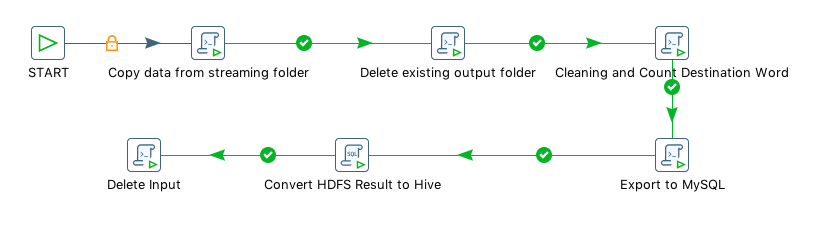
\includegraphics[scale=0.5]{Gambar/ui-implementation-pentaho-di.png}
	\caption[Implementasi ETL Job pada Pentaho Data Integration]{Implementasi ETL Job pada Pentaho Data Integration} 
	\label{fig:ui_implementation_pentaho_di}
\end{figure}

\subsection{Implementasi Modul Program Sistem Kecerdasan Bisnis}
Implementasi modul program sistem kecerdasan bisnis akan terbagi menjadi tiga buah bagian yaitu implementasi antarmuka program \textit{client} dan implementasi kode di sisi \textit{client} dan \textit{server}. 

\subsubsection{Implementasi Antarmuka Sistem Kecerdasan Bisnis}
Terdapat dua buah antarmuka yang diimplementasikan pada penelitian ini. Antarmuka yang pertama adalah antarmuka untuk halaman \textit{dashboard}. Pada halaman ini pengguna dapat melihat situasi tren lokasi wisata terkini. Gambar \ref{fig:ui_implementasi_bi_dashboard_1} menggambarkan kondisi awal ketika \textit{dashboard} diakses dan Gambar \ref{fig:ui_implementasi_bi_dashboard_2} menggambarkan kondisi \textit{drill down} ketika map dan diagram-diagram diklik.

\begin{figure}[H]
	\centering
	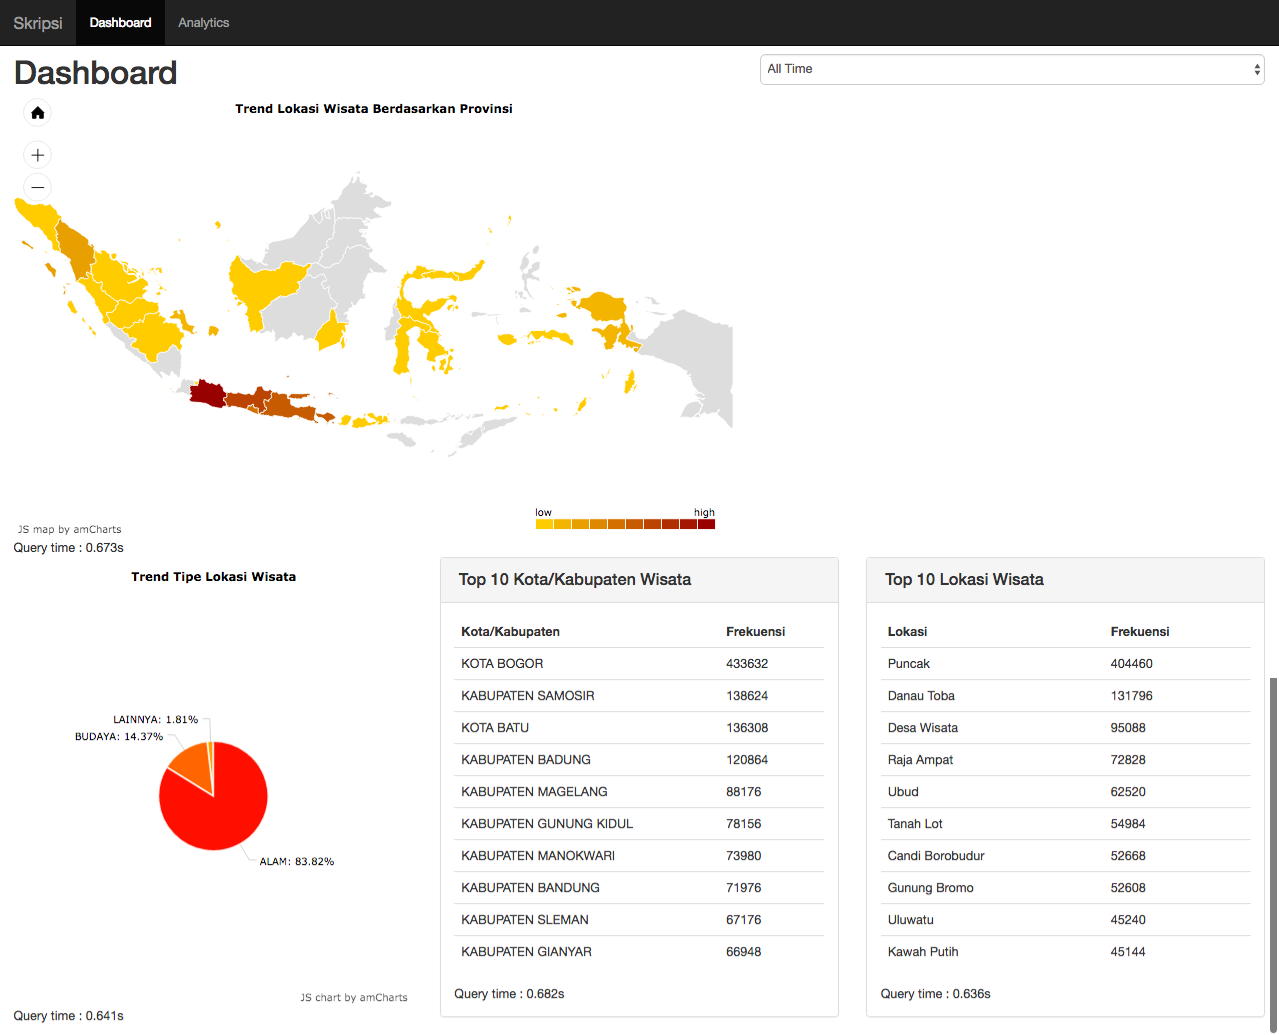
\includegraphics[scale=0.35]{Gambar/ui-implementasi-bi-dashboard-01.png}
	\caption[Implementasi Antarmuka Dashboard Sistem Kecerdasan Bisnis]{Implementasi Antarmuka Dashboard Sistem Kecerdasan Bisnis} 
	\label{fig:ui_implementasi_bi_dashboard_1}
\end{figure}

\begin{figure}[H]
	\centering
	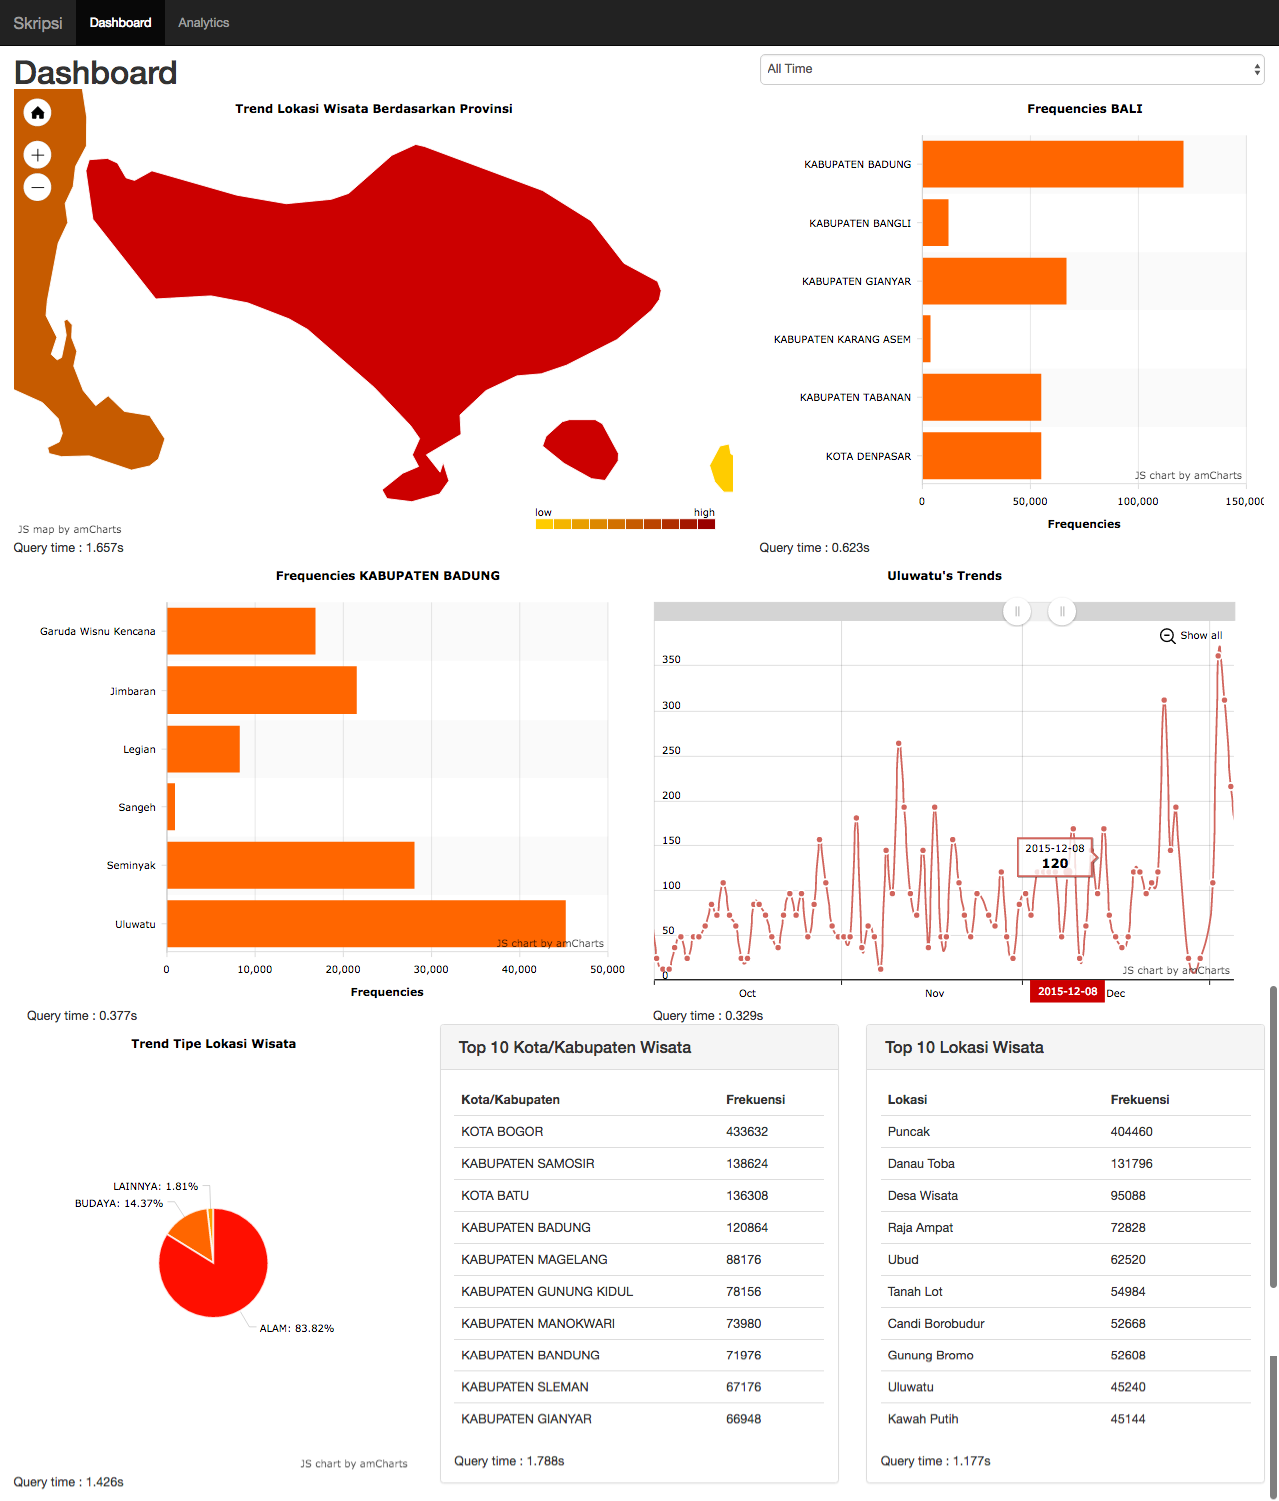
\includegraphics[scale=0.35]{Gambar/ui-implementasi-bi-dashboard-02.png}
	\caption[Implementasi Antarmuka Dashboard Sistem Kecerdasan Bisnis Ketika \textit{Drill Down}]{Implementasi Antarmuka Dashboard Sistem Kecerdasan Bisnis Ketika \textit{Drill Down}} 
	\label{fig:ui_implementasi_bi_dashboard_2}
\end{figure}

Antarmuka yang kedua adalah antarmuka untuk halaman pelaporan dan analisis. Pada halaman ini pengguna dapat memilih sumber data \textit{cube} yang hendak digunakan. Kemudian pengguna dapat melihat laporan dari berbagai sudut dimensi dan \textit{measure}. Terdapat juga pilihan untuk pengurutan data dan pembatasan jumlah data yang dicari. Pengguna juga bisa memasukan kriteria-kriteria yang diperlukan pada bagian \textit{filter} atau \textit{having}.

Tampilan data yang dihasilkan pada modul program ini dapat berupa tabel, diagram batang, diagram baris atau pun diagram pie. Contoh-contoh hasil tampilan data dari modul program ini terdapat pada Gambar \ref{fig:ui_implementasi_bi_reporting_1}, \ref{fig:ui_implementasi_bi_reporting_2}, dan \ref{fig:ui_implementasi_bi_reporting_3}.

\begin{figure}[H]
	\centering
	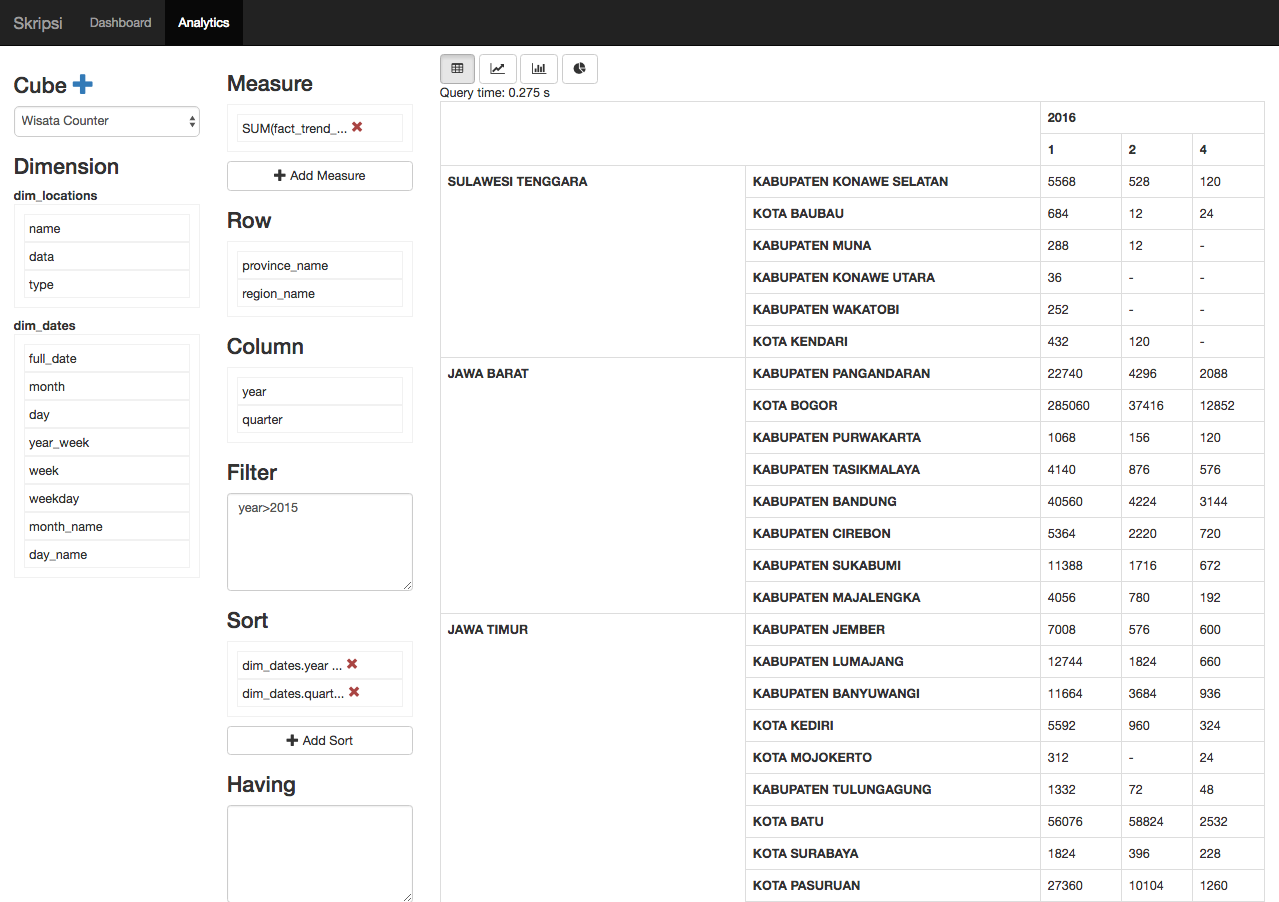
\includegraphics[scale=0.35]{Gambar/ui-implementasi-bi-reporting-01.png}
	\caption[Implementasi Antarmuka Tabel Pelaporan dan Analisis Sistem Kecerdasan Bisnis]{Implementasi Antarmuka Tabel Pelaporan dan Analisis Sistem Kecerdasan Bisnis} 
	\label{fig:ui_implementasi_bi_reporting_1}
\end{figure}

\begin{figure}[H]
	\centering
	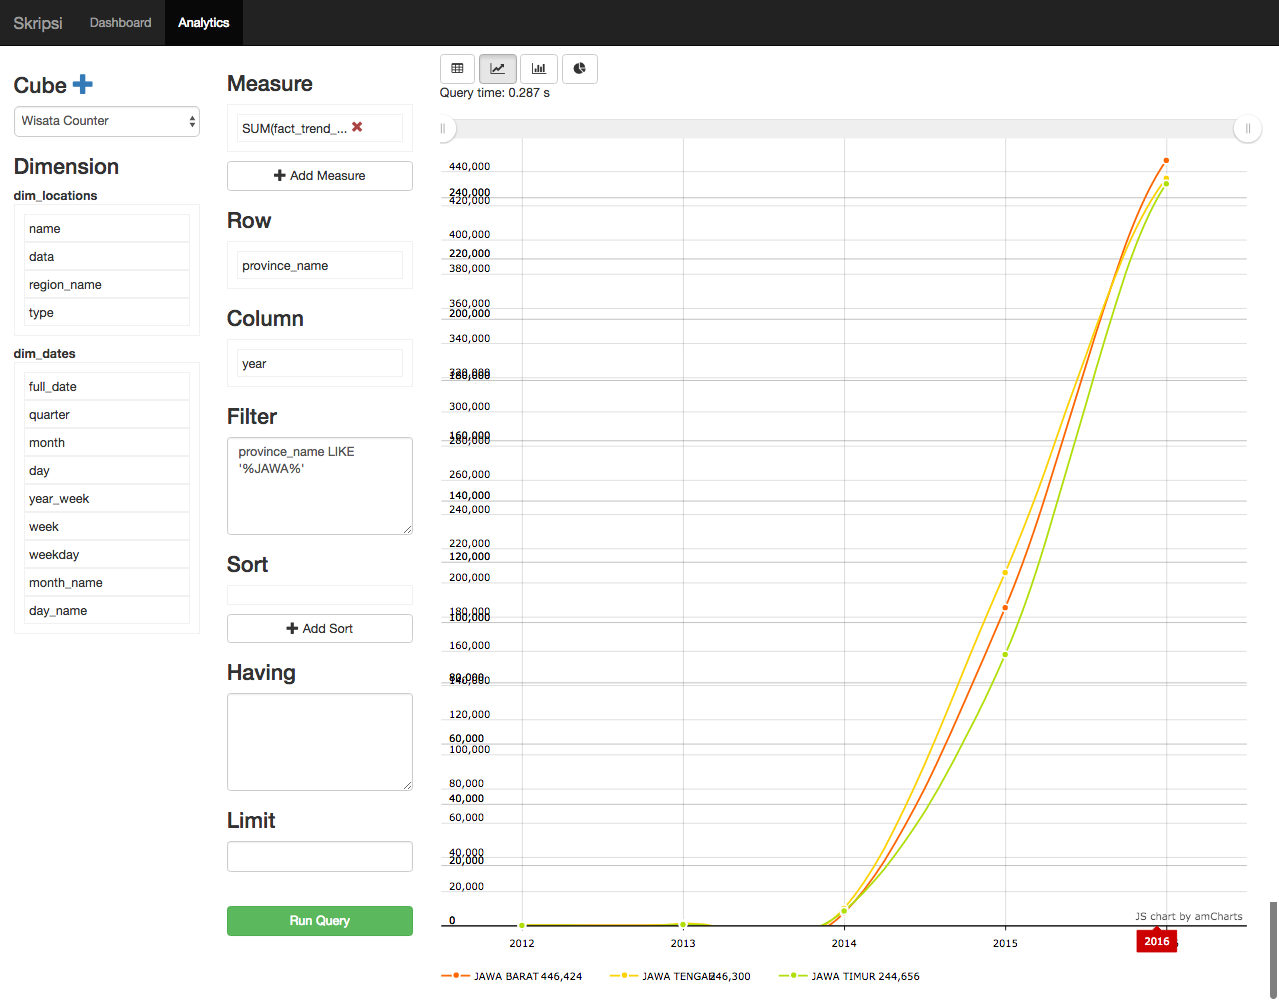
\includegraphics[scale=0.35]{Gambar/ui-implementasi-bi-reporting-02.png}
	\caption[Implementasi Antarmuka Grafik Pelaporan dan Analisis Sistem Kecerdasan Bisnis]{Implementasi Antarmuka Grafik Pelaporan dan Analisis Sistem Kecerdasan Bisnis} 
	\label{fig:ui_implementasi_bi_reporting_2}
\end{figure}

\begin{figure}[H]
	\centering
	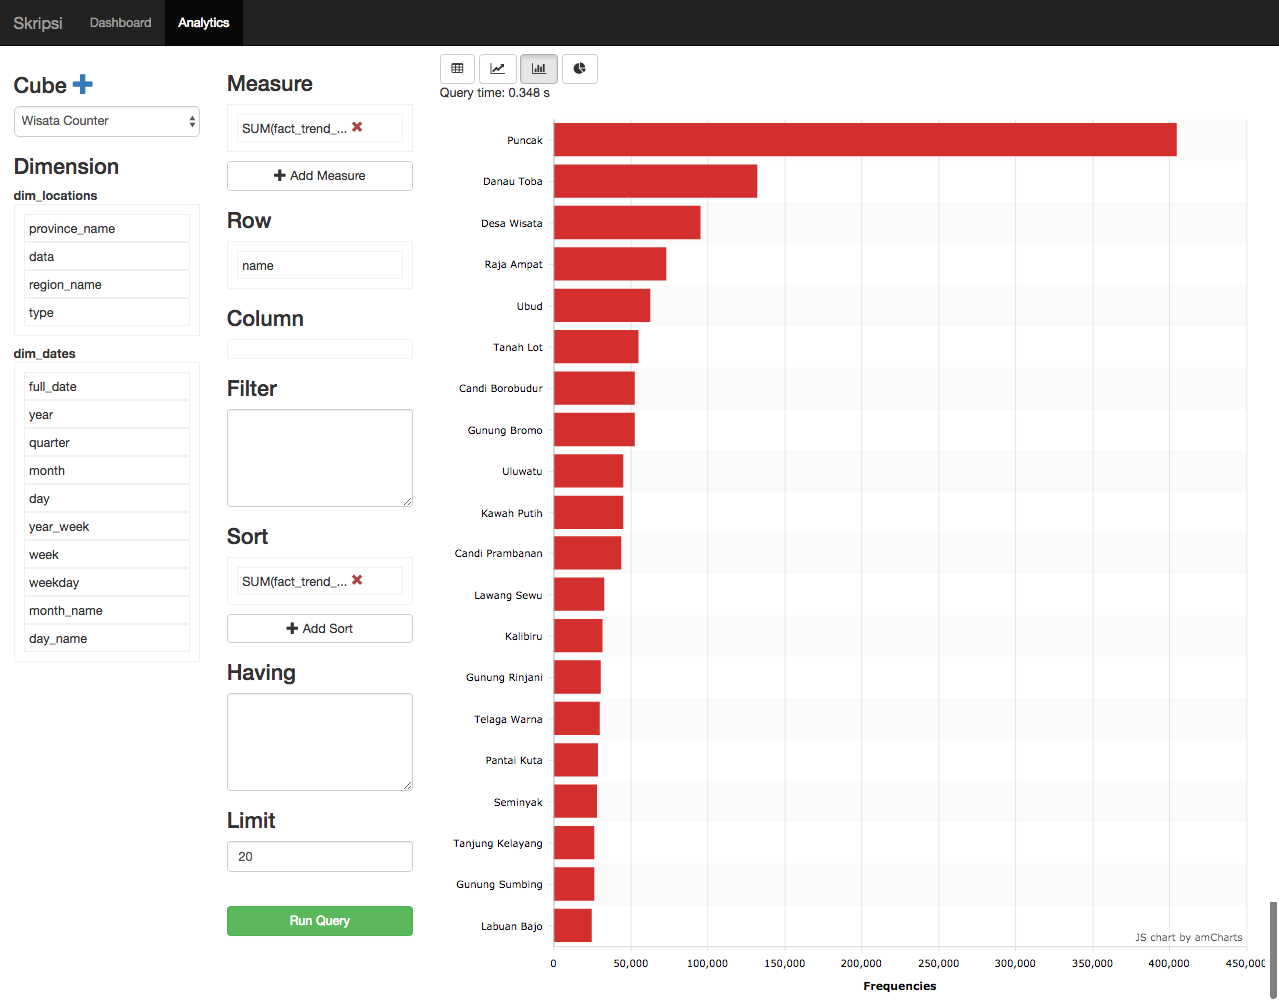
\includegraphics[scale=0.35]{Gambar/ui-implementasi-bi-reporting-03.png}
	\caption[Implementasi Antarmuka Grafik Pelaporan dan Analisis Sistem Kecerdasan Bisnis]{Implementasi Antarmuka Grafik Pelaporan dan Analisis Sistem Kecerdasan Bisnis} 
	\label{fig:ui_implementasi_bi_reporting_3}
\end{figure}

\subsubsection{Implementasi Kode Program Sistem Kecerdasan Bisnis}
Kode program pada sistem kecerdasan bisnis yang dibangun dibagi menjadi dua bagian. Bagian yang pertama adalah kode program di sisi \textit{client}, kode program pada bagian ini dibuat menggunakan HTML5, CSS, Javascript dan AMChart. Bagian yang kedua adalah kode program di sisi \textit{server}, kode program pada bagian ini dibuat dalam bahasa pemrograman Java dengan memanfaatkan Java servlet untuk melayani \textit{request} dan \textit{response} dari program \textit{client} via HTTP. 

Listing \ref{lst:kode_bi_client_dashboard_1}, \ref{lst:kode_bi_client_dashboard_2} dan \ref{lst:kode_bi_client_reporting_1} adalah potongan-potongan kode program dalam bahasa Javascript yang berjalan di sisi \textit{client}. Listing \ref{lst:kode_bi_client_dashboard_1} berfungsi untuk melakukan \textit{request} ke server kemudian menampilkan hasilnya ke dalam bentuk map menggunakan kode program pada Listing \ref{lst:kode_bi_client_dashboard_2}. Listing \ref{lst:kode_bi_client_reporting_1} berfungsi untuk mengirimkan \textit{request} ke server sesuai dengan kueri yang diinginkan oleh pengguna, \textit{response} pada listing ini akan ditampilkan dalam bentuk tabel.

Listing \ref{lst:kode_bi_server_reporting_1}, \ref{lst:kode_bi_server_reporting_2} dan \ref{lst:kode_bi_server_reporting_3} adalah potongan-potongan kode program di sisi server yang ditulis dalam bahasa Java. Listing \ref{lst:kode_bi_server_reporting_1} bertugas membuat koneksi ke sumber data, yaitu MySQL atau Hive. Listing \ref{lst:kode_bi_server_reporting_2} berfungsi untuk mengambil data dari \textit{connection file} lalu melakukan koneksi ke sumber data sesuai dengan konfigurasi di \textit{connection file}. Sedangkan pada Listing \ref{lst:kode_bi_server_reporting_3} berfungsi untuk membuat kueri-kueri yang sesuai dengan masukan dari pengguna.

\begin{lstlisting}[language=HTML,basicstyle=\tiny,caption=script-dasboard.js (Dashboard),label={lst:kode_bi_client_dashboard_1}]
....

$(function(){
    ....
    
    //load ajax
    var rowAttrs = "dim_locations.province_name,";
    var columnAttrs = "";
    var aggregate = "SUM(fact_trend_locations.qty),";
    var condition = "";
    var sort = "";
    var limit = 0;
    var having = "";

    $.ajax({
        method: "POST",
        url: baseUrl + "/generator",
        data: {rowAttrs: rowAttrs, columnAttrs: columnAttrs, aggregate: aggregate, condition: condition, sort: sort, limit: limit, having: having, connectionId: 1, cubeId: 0},
        success: function(data){
            globalMapData = data;
            createMap();
        },
        beforeSend: function(){
            $("#map").html("Loading...");
        }
    });
    
    ....
});

....
\end{lstlisting}

\begin{lstlisting}[language=HTML,basicstyle=\tiny,caption=script-dasboard.js (Dashboard),label={lst:kode_bi_client_dashboard_2}]
....
function createMap(){
    var areas = [];

    for (var i = 0; i < globalMapData.data.length; i++) {
        var data = globalMapData.data[i];
        var value = {};
        value['id'] = globalMaps[data.rows[0]];
        value['value'] = data.values[0];
        areas.push(value);
    }

    var map = new AmCharts.AmMap();
    map.titles = [{"text" : "Trend Lokasi Wisata Berdasarkan Provinsi"}]
    map.colorSteps = 10;
    map.dataProvider = {
        map: "indonesiaHigh",
        areas: areas
    };
    map.areasSettings = {
        autoZoom: true
    };
    map.imagesSettings.balloonText = "<span style='font-size:14px;'><b>[[title]]</b>: [[value]]</span>";

    var valueLegend = new AmCharts.ValueLegend();
    valueLegend.right = 20;
    valueLegend.minValue = "low";
    valueLegend.maxValue = "high";
    map.valueLegend = valueLegend;

    map.addListener("clickMapObject", clickGraph);
    map.write("map");

    $("#map-query-time").html("Query time : " + globalMapData.query_time / 1000 + "s");
}
....
\end{lstlisting}

\begin{lstlisting}[language=HTML,basicstyle=\tiny,caption=script.js (Membuat \textit{request} ke \textit{server} - Laporan dan Analisis),label={lst:kode_bi_client_reporting_1}]
....
$("#run-query").click(function(){
    var rowAttrs = "";
    var columnAttrs = "";
    var aggregate = "";
    var sort = "";
    var limit = 0;

    //get from measure
    $("#measure-sortable li").each(function(){
        aggregate += $(this).data("column") + ",";
    });

    //get from row
    $("#row-sortable li").each(function(){
        rowAttrs += $(this).data("column") + ",";
    });

    //get from column
    $("#column-sortable li").each(function(){
        columnAttrs += $(this).data("column") + ",";
    });

    //get sorting
    $("#sort-sortable li").each(function(){
        sort += $(this).data("column") + ",";
    });

    //get selected cube
    var option = $("#connection-select").find(":selected");

    //get limit
    if($("#limit").val() != "" && $("#limit").val() != 0){
        limit = $("#limit").val();
    }

    $.ajax({
        method: "POST",
        url: baseUrl + "/generator",
        data: {rowAttrs: rowAttrs, columnAttrs: columnAttrs, aggregate: aggregate, condition: $("#filter").val(), having: $("#having").val(), limit: limit, sort: sort, connectionId: option.data("connection"), cubeId: option.data("cube")},
        success: function(data){
       		if(data.data.length > 0){
                globalData = data;

                var resultOption = $("#result-option").find(".active").data("type");

                if(resultOption == "bar"){
                    createBarChart();
                }else if(resultOption == "line"){
                    createLineChart();
                }else if(resultOption == "table"){
                    generateTable();
                }else if(resultOption == "pie"){
                    createPieChart();
                }
            }else{
                $("#query-time").html("Query time: " + data.query_time / 1000 + "s");
                $("#result-area").html("No data found.");
            }
        },
        beforeSend: function(){
            $("#result-area").html("");
            $("#query-time").html("Loading...");
        }
    })
});
....
\end{lstlisting}

\begin{lstlisting}[language=Java,basicstyle=\tiny,caption=DbConnection.java,label={lst:kode_bi_server_reporting_1}]
public class DbConnection {
	....
	
    private static Connection con;
    
    public static Connection getConnection(String host, String user, String pass, int port, String db, String driver){
        try {
            String url = "";

            switch(driver){
                case "com.mysql.jdbc.Driver":
                    url = "jdbc:mysql://" + host + ":" + port + "/" + db + "";
                    break;
                case "org.apache.hive.jdbc.HiveDriver":
                    url = "jdbc:hive2://" + host + ":" + port + "/" + db + "";
                    break;
            }

            Class.forName(driver).newInstance();
            DbConnection.con = (Connection) DriverManager.getConnection(url, user, pass);
        } catch (Exception ex) {
            Logger.getLogger(DbConnection.class.getName()).log(Level.SEVERE, null, ex);
        } 
        
        return DbConnection.con;
    }
}
\end{lstlisting}

\begin{lstlisting}[language=Java,basicstyle=\tiny,caption=ConnectionReaderWriter.java,label={lst:kode_bi_server_reporting_2}]
public class ConnectionReaderWriter {
	... 
	
	public String getCubeDetail(int connectionId, int cubeId){
        try {
            JSONArray connections = new JSONArray(this.getConnections());
            JSONObject connection = (new JSONObject(this.getConnection(connectionId))).getJSONObject("connection");
            JSONObject cube = connections.getJSONObject(connectionId).getJSONArray("cubes").getJSONObject(cubeId);
            JSONArray dims = cube.getJSONArray("dim");
            
            String host = connection.getString("host");
            String user = connection.getString("username");
            String pass = connection.getString("password");
            String db = connection.getString("database");
            int port = connection.getInt("port");
            String driver = connection.getString("driver");
            
            conn = DbConnection.getConnection(host, user, pass, port, db, driver);
            String table = cube.getString("fact");
            
            //init json object as parent
            JSONObject json = new JSONObject();
            
            //fetch fact data
            JSONObject tableNodeJson = new JSONObject();
            tableNodeJson.put("name", table);
            tableNodeJson.put("columns", this.getColumn(table));            
            json.put("fact", tableNodeJson);
            
            //fetch dim data
            JSONArray dimsJson = new JSONArray();
            for (int i = 0; i < dims.length(); i++) {
                table = dims.getJSONObject(i).getString("table");
                tableNodeJson = new JSONObject();
                tableNodeJson.put("name", table);
                tableNodeJson.put("columns", this.getColumn(table)); 
                dimsJson.put(tableNodeJson);
            }
            json.put("dims", dimsJson);
            
            return json.toString();
        } catch (JSONException ex) {
            Logger.getLogger(ConnectionReaderWriter.class.getName()).log(Level.SEVERE, null, ex);
        } catch (IOException ex) {
            Logger.getLogger(ConnectionReaderWriter.class.getName()).log(Level.SEVERE, null, ex);
        } catch (SQLException ex) {
            Logger.getLogger(ConnectionReaderWriter.class.getName()).log(Level.SEVERE, null, ex);
        } 
        
        return null;
    }
    
    ...
}
\end{lstlisting}

\begin{lstlisting}[language=Java,basicstyle=\tiny,caption=QueryBuilder.java,label={lst:kode_bi_server_reporting_3}]
public class QueryBuilder {
    ....
    public String create(String rowAttrs, String columnAttrs , String aggregate, String condition, String order, int limit, String having){
        /**
         * SELECT ..., ..., SUM(...)
         * FROM fact
         * JOIN dim ON relation
         * JOIN dim ON relation
         * JOIN dim ON relation
         * WHERE ...
         * ORDER BY ... ASC
         * GROUP BY ..., ...
         */
        //set global so other methods can use it
        String attrs = (rowAttrs + columnAttrs);
        this.rowAttrs = rowAttrs;
        this.columnAttrs = columnAttrs;
        this.aggregate = aggregate;
        String sql = "SELECT ";
        //create select query
        sql += rowAttrs + columnAttrs;
        //create aggregate function
        sql += aggregate.substring(0, aggregate.length() - 1) + " ";
        //create from query
        sql += from + " ";
        //create join query
        sql += join + " ";
        //create where query
        if(condition != null && !condition.isEmpty()){
            sql += "WHERE " + condition + " ";
        }
        //create group query
        sql += "GROUP BY " + attrs.substring(0, attrs.length() - 1) + " ";
        
        if(having != null && !having.isEmpty()){
            sql += "HAVING " + having + " ";
        }
        
        //create order query
        if(!order.isEmpty()){
            sql += "ORDER BY " + order.substring(0, order.length() - 1) + " ";
        }
        if(limit != 0){
            sql += "LIMIT " + limit + " ";
        }
        
        return sql;
    }
    ....
}
\end{lstlisting}

\section{Pengujian Modul Program}
Pada sub bab ini, modul-modul program yang sudah dibuat akan diuji kebenaran berdasarkan masukan dan keluaran dari program. Tujuan dari pengujian ini adalah untuk memastikan bahwa setiap modul program sudah berjalan dengan benar sesuai dengan perancangan. Modul-modul program yang akan diuji adalah modul program untuk melakukan \textit{streaming} ke Twitter, \textit{crawling} Instagram serta modul program untuk menghitung tren lokasi wisata baik dengan MapReduce maupun tanpa MapReduce),.

\subsection{Pengujian Modul Program \textit{Streaming} Twitter}
Pengujian ini dilakukan untuk memastikan modul program yang dibuat dapat mengambil data dari Twitter Streaming API, serta menulis hasilnya ke HDFS. Pengujian ini di awali dengan memasukan consumer key, consumer secret, access token, dan access token secret yang didapat ketika mendaftarkan aplikasi di Twitter Streaming API. Kemudian dimasukan \textit{keyword-keyword} yang sesuai, yaitu libur, liburan, travel, travelling, wisata, tour, pariwisata, destinasi, jalan-jalan, hotel, pesawat, cruise, jelajah, petualangan. Untuk pilihan destinasi file dipilih HDFS dan diarahkan ke dalam path /wilianto/testing. 

\begin{figure}[H]
	\centering
	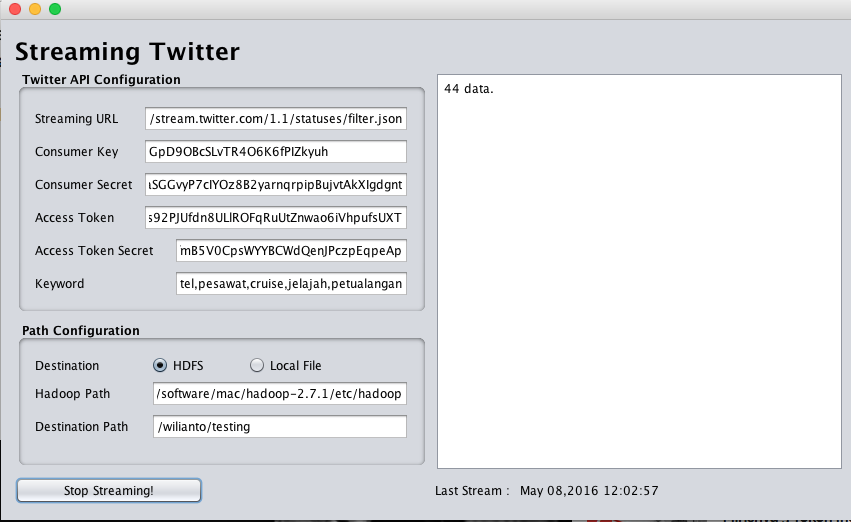
\includegraphics[scale=0.5]{Gambar/testing-twitter-01.png}
	\caption[Antar muka modul program ketika berjalan]{Antar muka modul program ketika berjalan} 
	\label{fig:testing_twitter_01}
\end{figure}

Setelah terisi maka \textit{streaming} ke Twitter dapat dilakukan. Tampilan antar muka program ketika sedang berproses dapat dilihat di Gambar \ref{fig:testing_twitter_01}. Hasil keluaran dari program di HDFS dapat dilihat pada Gambar \ref{fig:testing_twitter_02}. Berdasarkan pengujian ini maka, dapat disimpulkan modul program \textit{streaming} Twitter sudah berjalan dengan baik dan sesuai perancangan.

\begin{figure}[H]
	\centering
	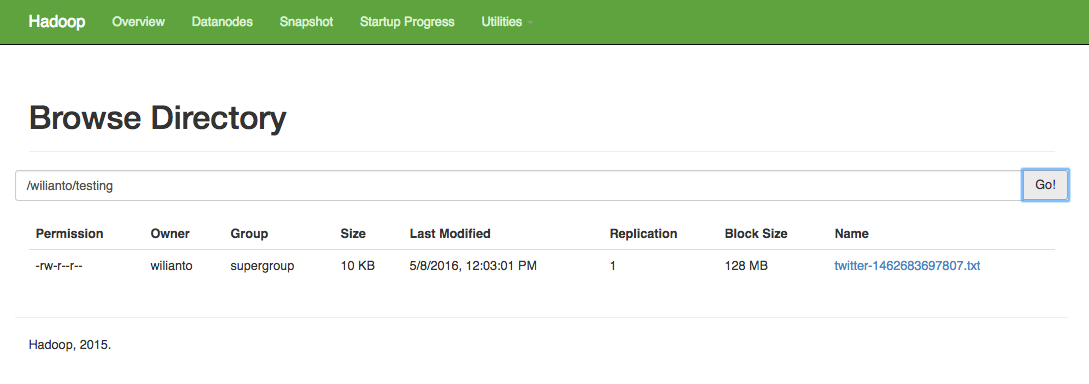
\includegraphics[scale=0.4]{Gambar/testing-twitter-02.png}
	\caption[Hasil keluaran dari modul program di HDFS]{Hasil keluaran dari modul program di HDFS} 
	\label{fig:testing_twitter_02}
\end{figure}

\subsection{Pengujian Modul Program \textit{Crawling} Instagram}
Pengujian ini dilakukan untuk memastikan modul program yang dibuat dapat mengambil data dari Instagram API, serta menulis hasilnya ke HDFS. Pengujian ini di awali dengan memasukan client ID, client secret dan redirect URL yang didapat ketika mendaftarkan aplikasi di Instagram API. Masukan berikutnya adalah code, untuk mendapatkan code pengguna harus mengklik tombol Get Code terlebih dahulu. Ketika tombol diklik, pengguna akan diarahkan ke browser dan diminta untuk melakukan autentikasi. Jika autentikasi berhasil dilakukan dan izin diberikan ke aplikasi, maka code akan diberikan. Pada masukan Next Min ID dapat dikosongkan apabila crawling ingin dilakukan dari data terbaru, sedangkan untuk melanjutkan dapat diisi dengan Next Min ID data awal. Tag yang diambil pada proses pengujian ini adalah exploreindonesia. Untuk pilihan destinasi file dipilih HDFS dan diarahkan ke dalam path /wilianto/testing. 

\begin{figure}[H]
	\centering
	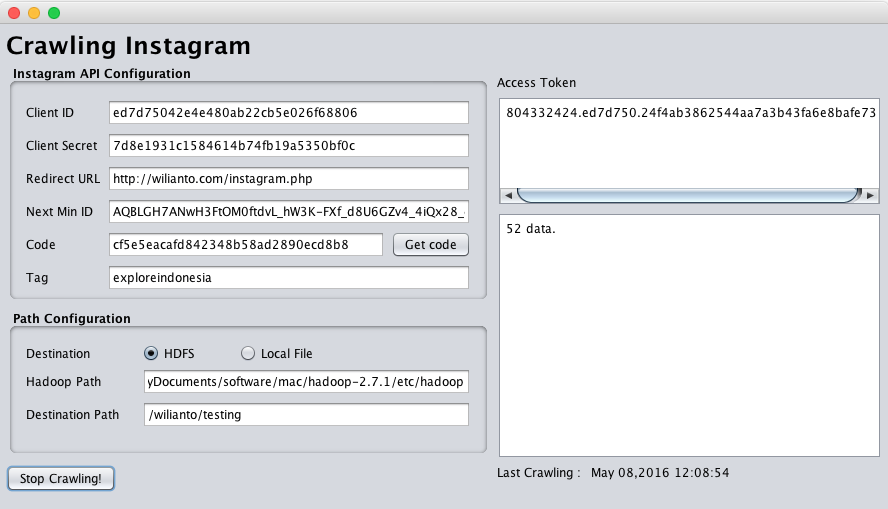
\includegraphics[scale=0.5]{Gambar/testing-instagram-01.png}
	\caption[Antar muka modul program ketika berjalan]{Antar muka modul program ketika berjalan} 
	\label{fig:testing_instagram_01}
\end{figure}

Setelah terisi maka \textit{crawling} ke Instagram dapat dilakukan. Tampilan antar muka program ketika sedang berproses dapat dilihat di Gambar \ref{fig:testing_instagram_01}. Hasil keluaran dari program di HDFS dapat dilihat pada Gambar \ref{fig:testing_instagram_02}. Berdasarkan pengujian ini maka, dapat disimpulkan modul program \textit{crawling} Instagram sudah berjalan dengan baik dan sesuai perancangan.

\begin{figure}[H]
	\centering
	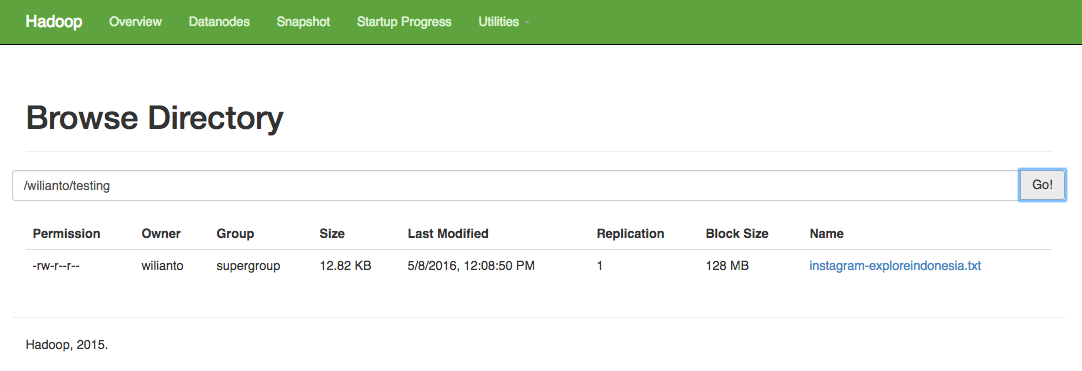
\includegraphics[scale=0.4]{Gambar/testing-instagram-02.png}
	\caption[Hasil keluaran dari modul program di HDFS]{Hasil keluaran dari modul program di HDFS} 
	\label{fig:testing_instagram_02}
\end{figure}

\subsection{Pengujian Modul Pembersihan Data dan Penghitungan Frekuensi Lokasi Wisata}
Pengujiannya dilakukan untuk memastikan modul program yang dibuat dapat melakukan pembersihan data dengan benar dan menghitung jumlah frekuensi kemunculan kata di dalam isi pesan sosial media (di kolom ke dua). Pada modul ini akan dilakukan pengujian dengan cara memasukan \textit{input} teks sosial media yang sudah dihitung secara manual jumlah kemunculan katanya. Lalu hasil keluaran dari program akan dicocokan dengan hasil perhitungan manual yang dilakukan. Hasil dari perhitungan manual dapat dilihat pada Tabel \ref{tab:hasil_hitung_manual} dan data input dapat dilihat pada Lampiran \ref{app:I}.

\begin{table}[!htb]
	\centering
	\begin{tabular}{| l | l | c |}
		\hline
		Lokasi & Tanggal & Frekuensi \\
	 	\hline
	 	candi borobudur & 2016-03-07 & 1\\
		candi borobudur & 2016-05-08 & 3\\
		dunia fantasi & 2016-05-08 & 2\\
		kawah putih & 2016-05-08 & 3\\
		pantai pangandaran & 2016-03-07 & 1\\
		pantai pangandaran & 2016-05-08 & 1\\
		pantai sanur & 2016-05-07 & 2\\
		pantai sanur & 2016-05-08 & 3\\
		pulau samosir & 2016-05-07 & 1\\
		pulau samosir & 2016-05-08 & 1\\
		pura besakih & 2016-05-08 & 1\\
		tanah lot & 2016-05-08 & 3\\
		tomok & 2016-05-08 & 1\\
		uluwatu & 2016-05-07 & 1\\
		uluwatu & 2016-05-08 & 1\\
	 	\hline
	\end{tabular}	
	\caption{Hasil Perhitungan Manual}\label{tab:hasil_hitung_manual}
\end{table}	

Hasil keluaran dari kedua program untuk pengujian ini dapat dilihat pada Gambar \ref{fig:counter_mp_output} untuk keluaran program dengan MapReduce dan Gambar \ref{fig:counter_single_output} untuk keluaran program tanpa MapReduce. Dari kedua keluaran dapat dilihat bahwa hasilnya sudah sesuai dengan perhitungan manual yang dilakukan. Oleh karena ini dapat ditarik kesimpulan bahwa modul program ini sudah berjalan dengan baik dan sesuai dengan perancangan.

\begin{figure}[H]
	\centering
	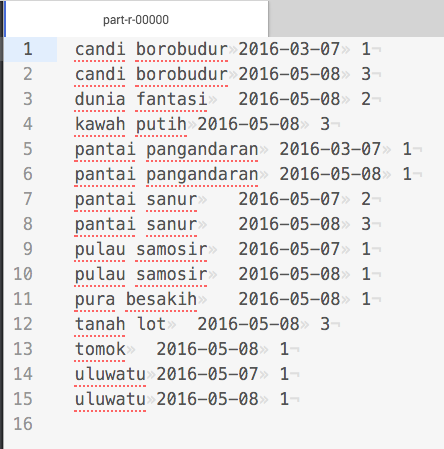
\includegraphics[scale=0.5]{Gambar/counter-mp-output.png}
	\caption[Hasil keluaran dari modul program dengan MapReduce]{Hasil keluaran dari modul program dengan MapReduce} 
	\label{fig:counter_mp_output}
\end{figure}

\begin{figure}[H]
	\centering
	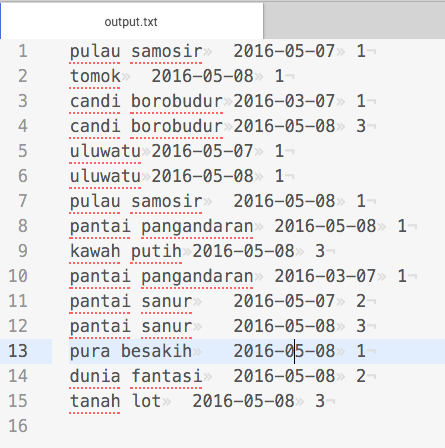
\includegraphics[scale=0.5]{Gambar/counter-single-output.png}
	\caption[Hasil keluaran dari modul program tanpa MapReduce]{Hasil keluaran dari modul program tanpa MapReduce} 
	\label{fig:counter_single_output}
\end{figure}

\section{Eksperimen}
Pengujian waktu eksekusi program dilakukan untuk mengukur kecepatan program dalam menyelesaikan masalah. Pengujian dilakukan pada dua modul program yang berbeda, yaitu modul program untuk pembersihan dan menghitung frekuensi kemunculan lokasi wisata. Pengujian kedua dilakukan pada modul program sistem kecerdasan bisnis untuk menghitung kecepatan kueri-kueri yang dibuat.

Dalam melakukan pengujian, penguji menggunakan komputer-komputer di dalam laboratorium sesuai dengan spesifikasi yang sudah dijelaskan pada Bab \ref{sec:deskripsi_perangkat_keras}. Terdapat dua buah pengujian yang dilakukan untuk modul program pembersihan dan menghitung frekuensi, yaitu pengaruh ukuran blok terhadap waktu eksekusi dan pengaruh jumlah node terhadap waktu eksekusi.

\subsection{Uji Pengaruh Ukuran Blok terhadap Kecepatan}
Pengujian pengaruh ukuran blok terhadap waktu dilakukan dengan spesifikasi seperti berikut: 
\begin{itemize}
	\item Jumlah node: 25 node
	\item Ukuran data: 10.98 GB (terdiri dari data tweet dan caption instagram yang sudah diduplikasi)
\end{itemize}

\begin{table}
	\centering
	\begin{tabular}{| l | c | c | c | c | c | c |}
		\hline
		Block Size (MB)	& 1 & 2 & 3 & 4 & 5 & Rata-rata  \\
		\hline
		16 	& 122	& 119	& 118	& 118	& 117  & 118.8 \\
		32		& 88	& 84	& 83	& 87	& 82 & 84.8\\
		64		& 67	& 65	& 67	& 66	& 65 & 66\\
		128	& 66	& 59	& 61	& 57	& 58 & 60.2\\
		\hline
	\end{tabular}	
	\caption{Hasil uji pengaruh ukuran blok terhadap kecepatan dalam detik} \label{tab:waktu_blok}
\end{table}	

Gambar \ref{fig:eks_block_size} memperlihatkan grafik rata-rata waktu ekskusi. Dari grafik dapat dilihat bahwa ukuran blok memiliki pengaruh terhadap waktu eksekusi program. Waktu eksekusi tercepat adalah pada ukuran blok 128 MB.

\begin{figure}[H]
	\centering
	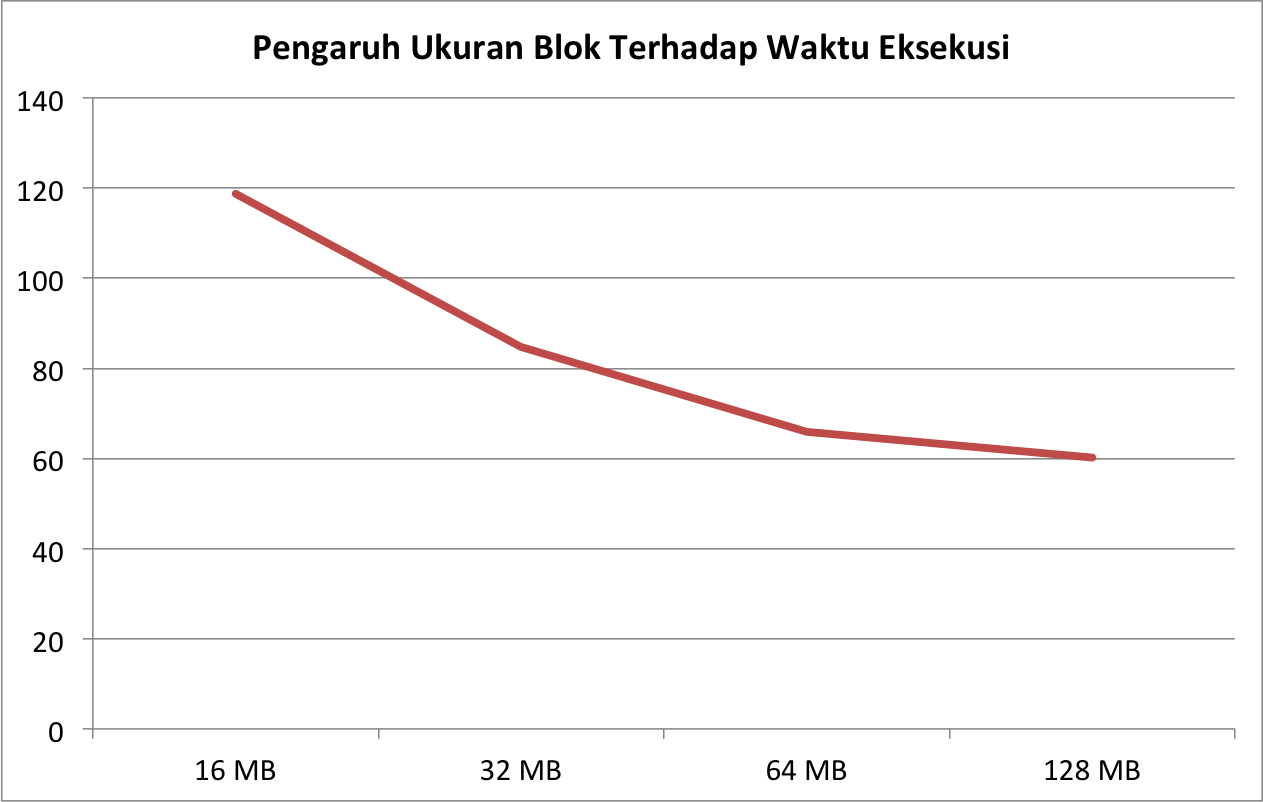
\includegraphics[scale=0.5]{Gambar/eks-block-size.png}
	\caption[Grafik pengaruh ukuran blok terhadap rata-rata waktu eksekusi]{Grafik pengaruh ukuran blok terhadap rata-rata waktu eksekusi} 
	\label{fig:eks_block_size}
\end{figure}

\subsection{Uji Pengaruh Jumlah Node terhadap Kecepatan}
Pengujian berikutnya adalah pengujian pengaruh jumlah \textit{node} terhadap waktu eksekusi. Pada pengujian ini, jumlah \textit{node} yang digunakan adalah kelipatan 5, dimulai dengan 1 node terlebih dahulu. Selain itu pengujian kali ini menguji performa modul program tanpa MapReduce. Hasil pengujian tertera pada Tabel \ref{tab:waktu_node}. Spesifikasi komputer-komputer yang digunakan pada pengujian ini adalah:
\begin{itemize}
	\item Jumlah node: mulai dari 1 hingga 25 
	\item Ukuran data: 10.98 GB (terdiri dari data tweet dan caption instagram yang sudah diduplikasi)
	\item Ukuran blok: 128 MB
\end{itemize}

\begin{table}
	\centering
	\begin{tabular}{ | l | c | c | c | c | c | c |}
		\hline
		Jumlah Node	& 1 & 2 & 3 & 4 & 5 & Rata-rata  \\
		\hline
		Tanpa MapReduce & 958	& 953	& 955	& 950	& 948  & 952.8\\
		1	& 1015	& 1012	& 1005	& 1008	& 1010 & 1010\\
		5	& 210	& 202	& 201	& 200	& 201 & 202.8\\
		10	 & 120	& 113	& 112	& 117	& 119 & 116.2\\
		15	 & 99	 & 99 & 98	 & 97 	& 93  & 97.2\\
		20	 & 75	 & 77 & 80	 & 69	 & 70 & 74.2\\
		25	 & 66	 & 59	 & 61 & 57	 & 58 & 60.2\\
		\hline
	\end{tabular}	
	\caption{Hasil uji pengaruh jumlah node terhadap kecepatan program dalam detik}\label{tab:waktu_node}
\end{table}	

Pada Gambar \ref{fig:eks_node_size} terlihat bahwa jumlah \textit{node} memiliki dampak pada kecepatan waktu eksekusi.

\begin{figure}[H]
	\centering
	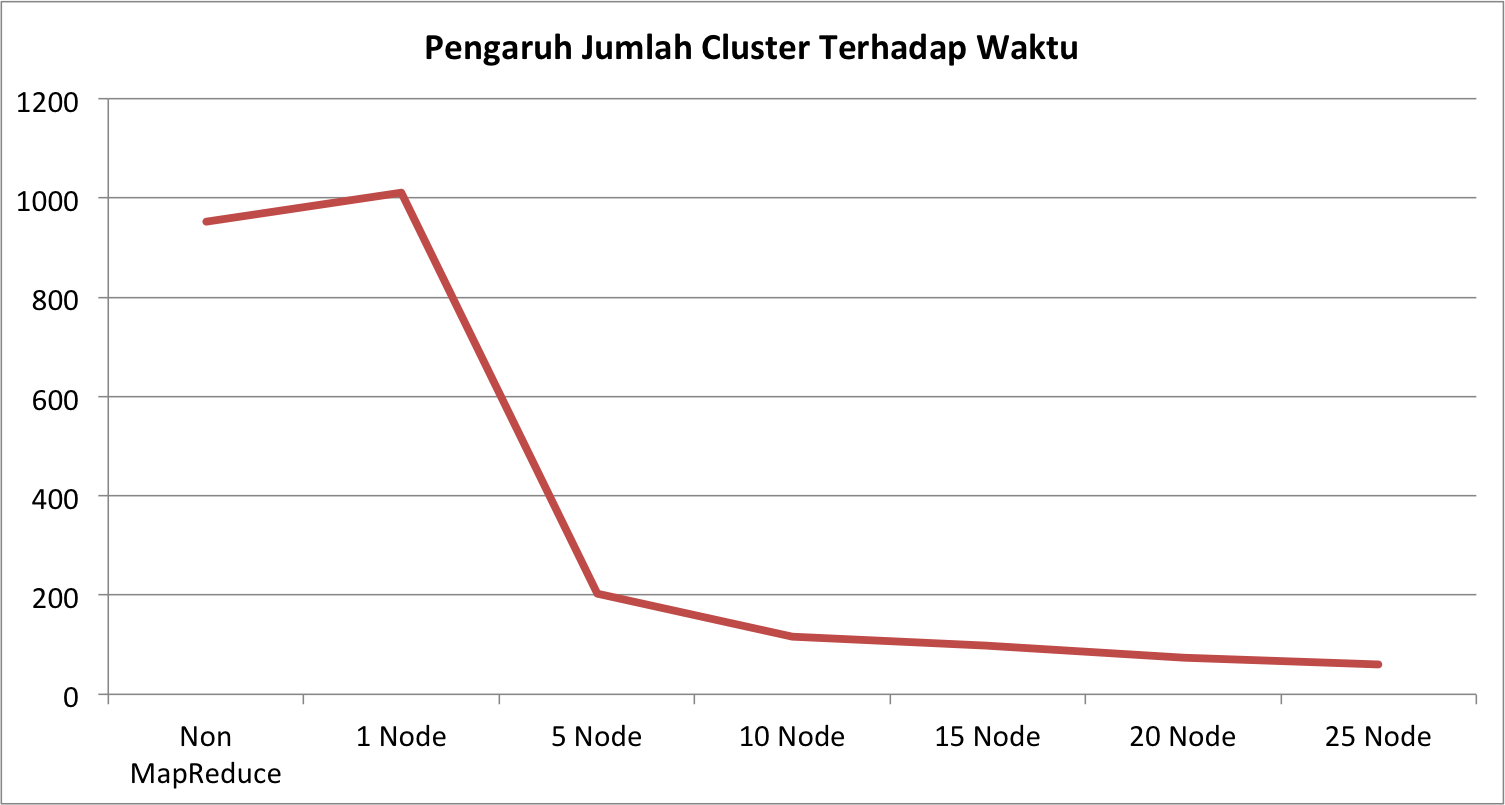
\includegraphics[scale=0.5]{Gambar/eks-node-size.png}
	\caption[Grafik pengaruh jumlah node terhadap rata-rata waktu eksekusi]{Grafik pengaruh jumlah node terhadap rata-rata waktu eksekusi} 
	\label{fig:eks_node_size}
\end{figure}

\subsection{Eksperimen Kueri}
Pengujian kedua dilakukan pada modul program sistem kecerdasan bisnis untuk menghitung kecepatan kueri-kueri yang dibuat. Pengujian dilakukan dengan membandingkan performa kueri yang dijalankan pada Hive dan pada MySQL. Pada pengujian ini digunakan komputer-komputer dengan spesifikasi sebagai berikut untuk menjalankan kueri-kueri di Hive.
\begin{itemize}
	\item Jumlah node: 25 
	\item Ukuran data: 32.867.328 (dengan duplikasi dari hasil keluaran MapReduce)
	\item Ukuran blok: 128 MB
	\item Processor: 3.3 GHz Intel Core i3
	\item RAM: 4 GB DDR3
	\item Sistem Operasi: Ubuntu 14.04 LTS
	\item Versi Java: 1.8.0\_45
\end{itemize}

Sedangkan untuk MySQL menggunakan sebuah komputer dengan spesifikasi sebagai berikut:
\begin{enumerate}
	\item Processor: 3.3 GHz Intel Core i3
	\item RAM: 4 GB DDR3
	\item Sistem Operasi: Ubuntu 14.04 LTS
	\item Versi Java: 1.8.0\_45
\end{enumerate}

Listing \ref{lst:kueri_1}, \ref{lst:kueri_2}, \ref{lst:kueri_3} dan \ref{lst:kueri_4} adalah kueri-kueri yang diuji.

\begin{lstlisting}[language=SQL,basicstyle=\tiny,caption=Mencari tren wisata per provinsi,label={lst:kueri_1}]
SELECT dim_locations.province_name,SUM(fact_trend_locations.qty) 
FROM fact_trend_locations 
INNER JOIN dim_locations ON dim_locations.name = fact_trend_locations.destination 
LEFT JOIN dim_dates ON dim_dates.full_date = fact_trend_locations.post_date  
GROUP BY dim_locations.province_name 
\end{lstlisting}

\begin{lstlisting}[language=SQL,basicstyle=\tiny,caption=Mencari tren suatu lokasi wisata dari bulan ke bulan,label={lst:kueri_2}]
SELECT dim_locations.name,dim_dates.year,dim_dates.month,SUM(fact_trend_locations.qty) 
FROM fact_trend_locations 
INNER JOIN dim_locations ON dim_locations.name = fact_trend_locations.destination 
LEFT JOIN dim_dates ON dim_dates.full_date = fact_trend_locations.post_date  
WHERE dim_locations.name='danau toba' 
GROUP BY dim_locations.name,dim_dates.year,dim_dates.month 
ORDER BY dim_dates.year ASC,dim_dates.month ASC 
\end{lstlisting}

\begin{lstlisting}[language=SQL,basicstyle=\tiny,caption=Mencari tren suatu lokasi wisata dari hari ke hari,label={lst:kueri_3}]
SELECT dim_locations.name,dim_dates.year,dim_dates.month,dim_dates.day,SUM(fact_trend_locations.qty) 
FROM fact_trend_locations 
INNER JOIN dim_locations ON dim_locations.name = fact_trend_locations.destination 
LEFT JOIN dim_dates ON dim_dates.full_date = fact_trend_locations.post_date  
WHERE dim_locations.name='danau toba' 
GROUP BY dim_locations.name,dim_dates.year,dim_dates.month,dim_dates.day 
ORDER BY dim_dates.year ASC,dim_dates.month ASC,dim_dates.day ASC 
\end{lstlisting}

\begin{lstlisting}[language=SQL,basicstyle=\tiny,caption=Mencari tren tipe lokasi wisata,label={lst:kueri_4}]
SELECT dim_locations.type,SUM(fact_trend_locations.qty) 
FROM fact_trend_locations 
INNER JOIN dim_locations ON dim_locations.name = fact_trend_locations.destination 
LEFT JOIN dim_dates ON dim_dates.full_date = fact_trend_locations.post_date  
GROUP BY dim_locations.type 
\end{lstlisting}

Hasil dari pengujian ini dapat dilihat pada Tabel \ref{tab:eks_kueri}. Terdapat perbedaan waktu eksekusi kueri pada Hive dan MySQL.

\begin{table}
	\centering
	\begin{tabular}{| l | c | c |}
		\hline
		Kueri	& MySQL & Hive  \\
		\hline
		Listing \ref{lst:kueri_1} & 138.88 & 70.928 \\
		Listing \ref{lst:kueri_2} & 115.308 & 100.361 \\
		Listing \ref{lst:kueri_3} & 120.752 & 55.067 \\
		Listing \ref{lst:kueri_4} & 155.535 & 50.743 \\
		\hline
	\end{tabular}	
	\caption{Waktu eksekusi kueri-kueri dalam detik}\label{tab:eks_kueri}
\end{table}	

\section{Kesimpulan Eksperimen}
Berdasarkan pengujian-pengujian yang telah dilakukan, maka dapat diambil kesimpulan sebagai berikut:

\begin{itemize}
	\item Ukuran blok berpengaruh pada performa kecepatan eksekusi dari program yang dijalakan. Oleh karena itu pemilihan ukuran blok yang tepat perlu dilakukan dengan baik, agar program yang dieksekusi dapat berjalan secara optimal.
	\item Jumlah \textit{node} sangat berpengaruh pada kecepatan eksekusi program. Program MapReduce menghasilkan performa yang lebih baik apabila jumlah \textit{node}-nya banyak. Sedangkan jika hanya 1 node saja, maka waktu eksekusi program MapReduce lebih lambat daripada program Java tanpa menggunakan MapReduce.
	\item Kueri-kueri yang dijalankan di Hive memiliki performa yang lebih cepat dibandingkan kueri-kueri yang dijalankan pada MySQL.
\end{itemize}